


\tikzset{every picture/.style={line width=0.75pt}} %set default line width to 0.75pt        

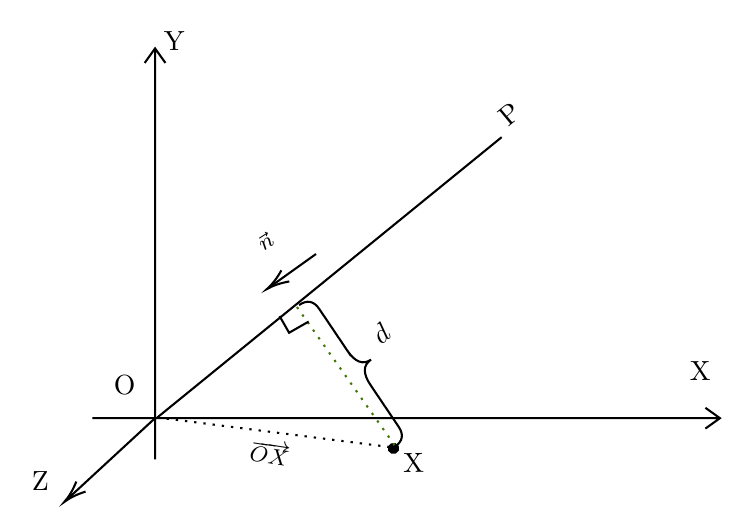
\begin{tikzpicture}[x=0.75pt,y=0.75pt,yscale=-1,xscale=1]
%uncomment if require: \path (0,263); %set diagram left start at 0, and has height of 263

%Shape: Axis 2D [id:dp44317292301248945] 
\draw  (166.5,203.07) -- (468.9,203.07)(196.74,24.92) -- (196.74,222.87) (461.9,198.07) -- (468.9,203.07) -- (461.9,208.07) (191.74,31.92) -- (196.74,24.92) -- (201.74,31.92)  ;
%Straight Lines [id:da2979242010824248] 
\draw    (197.86,202.72) -- (363.74,67.68) ;
%Shape: Ellipse [id:dp023999541748674025] 
\draw  [fill={rgb, 255:red, 0; green, 0; blue, 0 }  ,fill opacity=1 ] (310.87,219.7) .. controls (309.68,219.31) and (309.04,218.07) .. (309.45,216.93) .. controls (309.86,215.8) and (311.16,215.19) .. (312.35,215.58) .. controls (313.54,215.97) and (314.17,217.21) .. (313.76,218.35) .. controls (313.35,219.48) and (312.06,220.09) .. (310.87,219.7) -- cycle ;
%Straight Lines [id:da4396600304527325] 
\draw    (274.28,123.97) -- (252.25,139.71) ;
\draw [shift={(250.62,140.87)}, rotate = 324.46] [color={rgb, 255:red, 0; green, 0; blue, 0 }  ][line width=0.75]    (10.93,-3.29) .. controls (6.95,-1.4) and (3.31,-0.3) .. (0,0) .. controls (3.31,0.3) and (6.95,1.4) .. (10.93,3.29)   ;
%Straight Lines [id:da11083812462923981] 
\draw  [dash pattern={on 0.84pt off 2.51pt}]  (197.86,202.72) -- (309.45,216.93) ;
%Straight Lines [id:da3033500048537672] 
\draw [color={rgb, 255:red, 65; green, 117; blue, 5 }  ,draw opacity=1 ] [dash pattern={on 0.84pt off 2.51pt}]  (265.1,149.52) -- (313.76,218.35) ;
%Shape: Brace [id:dp9223930624399752] 
\draw   (312.19,216.89) .. controls (316.06,214.28) and (316.69,211.04) .. (314.08,207.17) -- (300.55,187.1) .. controls (296.82,181.57) and (296.9,177.51) .. (300.77,174.9) .. controls (296.9,177.51) and (293.1,176.05) .. (289.37,170.52)(291.05,173) -- (275.85,150.45) .. controls (273.24,146.58) and (270,145.95) .. (266.13,148.56) ;
%Straight Lines [id:da5740957717017106] 
\draw    (256.74,153.91) -- (261.33,161.91) -- (270.72,156.55) ;
%Straight Lines [id:da9385906535715354] 
\draw    (196.74,203.07) -- (154.47,242.1) ;
\draw [shift={(153,243.45)}, rotate = 317.29] [color={rgb, 255:red, 0; green, 0; blue, 0 }  ][line width=0.75]    (10.93,-3.29) .. controls (6.95,-1.4) and (3.31,-0.3) .. (0,0) .. controls (3.31,0.3) and (6.95,1.4) .. (10.93,3.29)   ;

% Text Node
\draw (175.39,180.91) node [anchor=north west][inner sep=0.75pt]   [align=left] {O};
% Text Node
\draw (358.93,55.68) node [anchor=north west][inner sep=0.75pt]  [rotate=-320.43] [align=left] {P};
% Text Node
\draw (314.8,218.52) node [anchor=north west][inner sep=0.75pt]  [rotate=-359.39] [align=left] {X};
% Text Node
\draw (242.82,116.02) node [anchor=north west][inner sep=0.75pt]  [font=\footnotesize,rotate=-327.31]  {$\vec{n}$};
% Text Node
\draw (297.75,160.53) node [anchor=north west][inner sep=0.75pt]  [rotate=-321.21]  {$d$};
% Text Node
\draw (242.17,211.95) node [anchor=north west][inner sep=0.75pt]  [font=\footnotesize,rotate=-8.77]  {$\overrightarrow{OX}$};
% Text Node
\draw (452.87,174.47) node [anchor=north west][inner sep=0.75pt]   [align=left] {X};
% Text Node
\draw (199.49,15.43) node [anchor=north west][inner sep=0.75pt]   [align=left] {Y};
% Text Node
\draw (135.87,227.47) node [anchor=north west][inner sep=0.75pt]   [align=left] {Z};


\end{tikzpicture}